\begin{frame}
  \frametitle{¿Cómo escoger el mejor material de forma objetiva?}
  \begin{block}{Los Diagramas de Ashby: El Concepto}
    Este método, revolucionario en ingeniería, permite sistematizar la selección
    de materiales.

    \begin{itemize}
      \item Se basa en una \textbf{ecuación de rendimiento (P)} que describe el
        desempeño de un componente.
      \item Esta ecuación relaciona los requisitos funcionales (F), la geometría
        (G) y las \textbf{propiedades del material (M)}.
        $$ P = f(F, G, M) $$
    \end{itemize}
  \end{block}
\end{frame}

\begin{frame}
  \frametitle{Aislar las Propiedades del Material}
  \begin{block}{El Objetivo del Método}
    \begin{itemize}
      \item El truco consiste en reordenar la ecuación de rendimiento para
        \textbf{aislar todas las propiedades del material (M)} en un único
        término.
        $$ (\text{Rendimiento}) = (\text{Función}) \cdot (\text{Geometría})
        \cdot (\textbf{Material}) $$
      \item Este término de \textbf{Material} se convierte en el \textbf{Índice
        de Material ($\mathcal{M}$)}.
      \item Al maximizar este índice, podemos encontrar el candidato ideal de
        forma objetiva, eliminando los sesgos del diseñador.
    \end{itemize}
  \end{block}
\end{frame}

\begin{frame}
  \frametitle{¿Por Qué Minimizar el Espesor en Fusión?}
  \begin{block}{El Desafío del Tokamak Esférico}
    En un reactor de fusión tipo tokamak, el blindaje de la columna central es
    uno de los componentes más críticos.
    \begin{itemize}
      \item El rendimiento y la potencia del reactor son \textbf{inversamente
        proporcionales} al grosor de este blindaje.
      \item Un blindaje más delgado permite un campo magnético más fuerte, lo
        que resulta en un reactor más eficiente y potente.
      \item Por lo tanto, el objetivo principal es encontrar un material que
        ofrezca la máxima protección en el \textbf{mínimo espacio posible}.
    \end{itemize}
  \end{block}
  \begin{block}{Índice de Material a Optimizar}
    Para este problema, maximizamos el índice de espesor mínimo:
    $ \mathcal{M}_{1} = N \cdot \lambda_{eff} $
  \end{block}
\end{frame}

\begin{frame}
  \begin{figure}
    \centering
    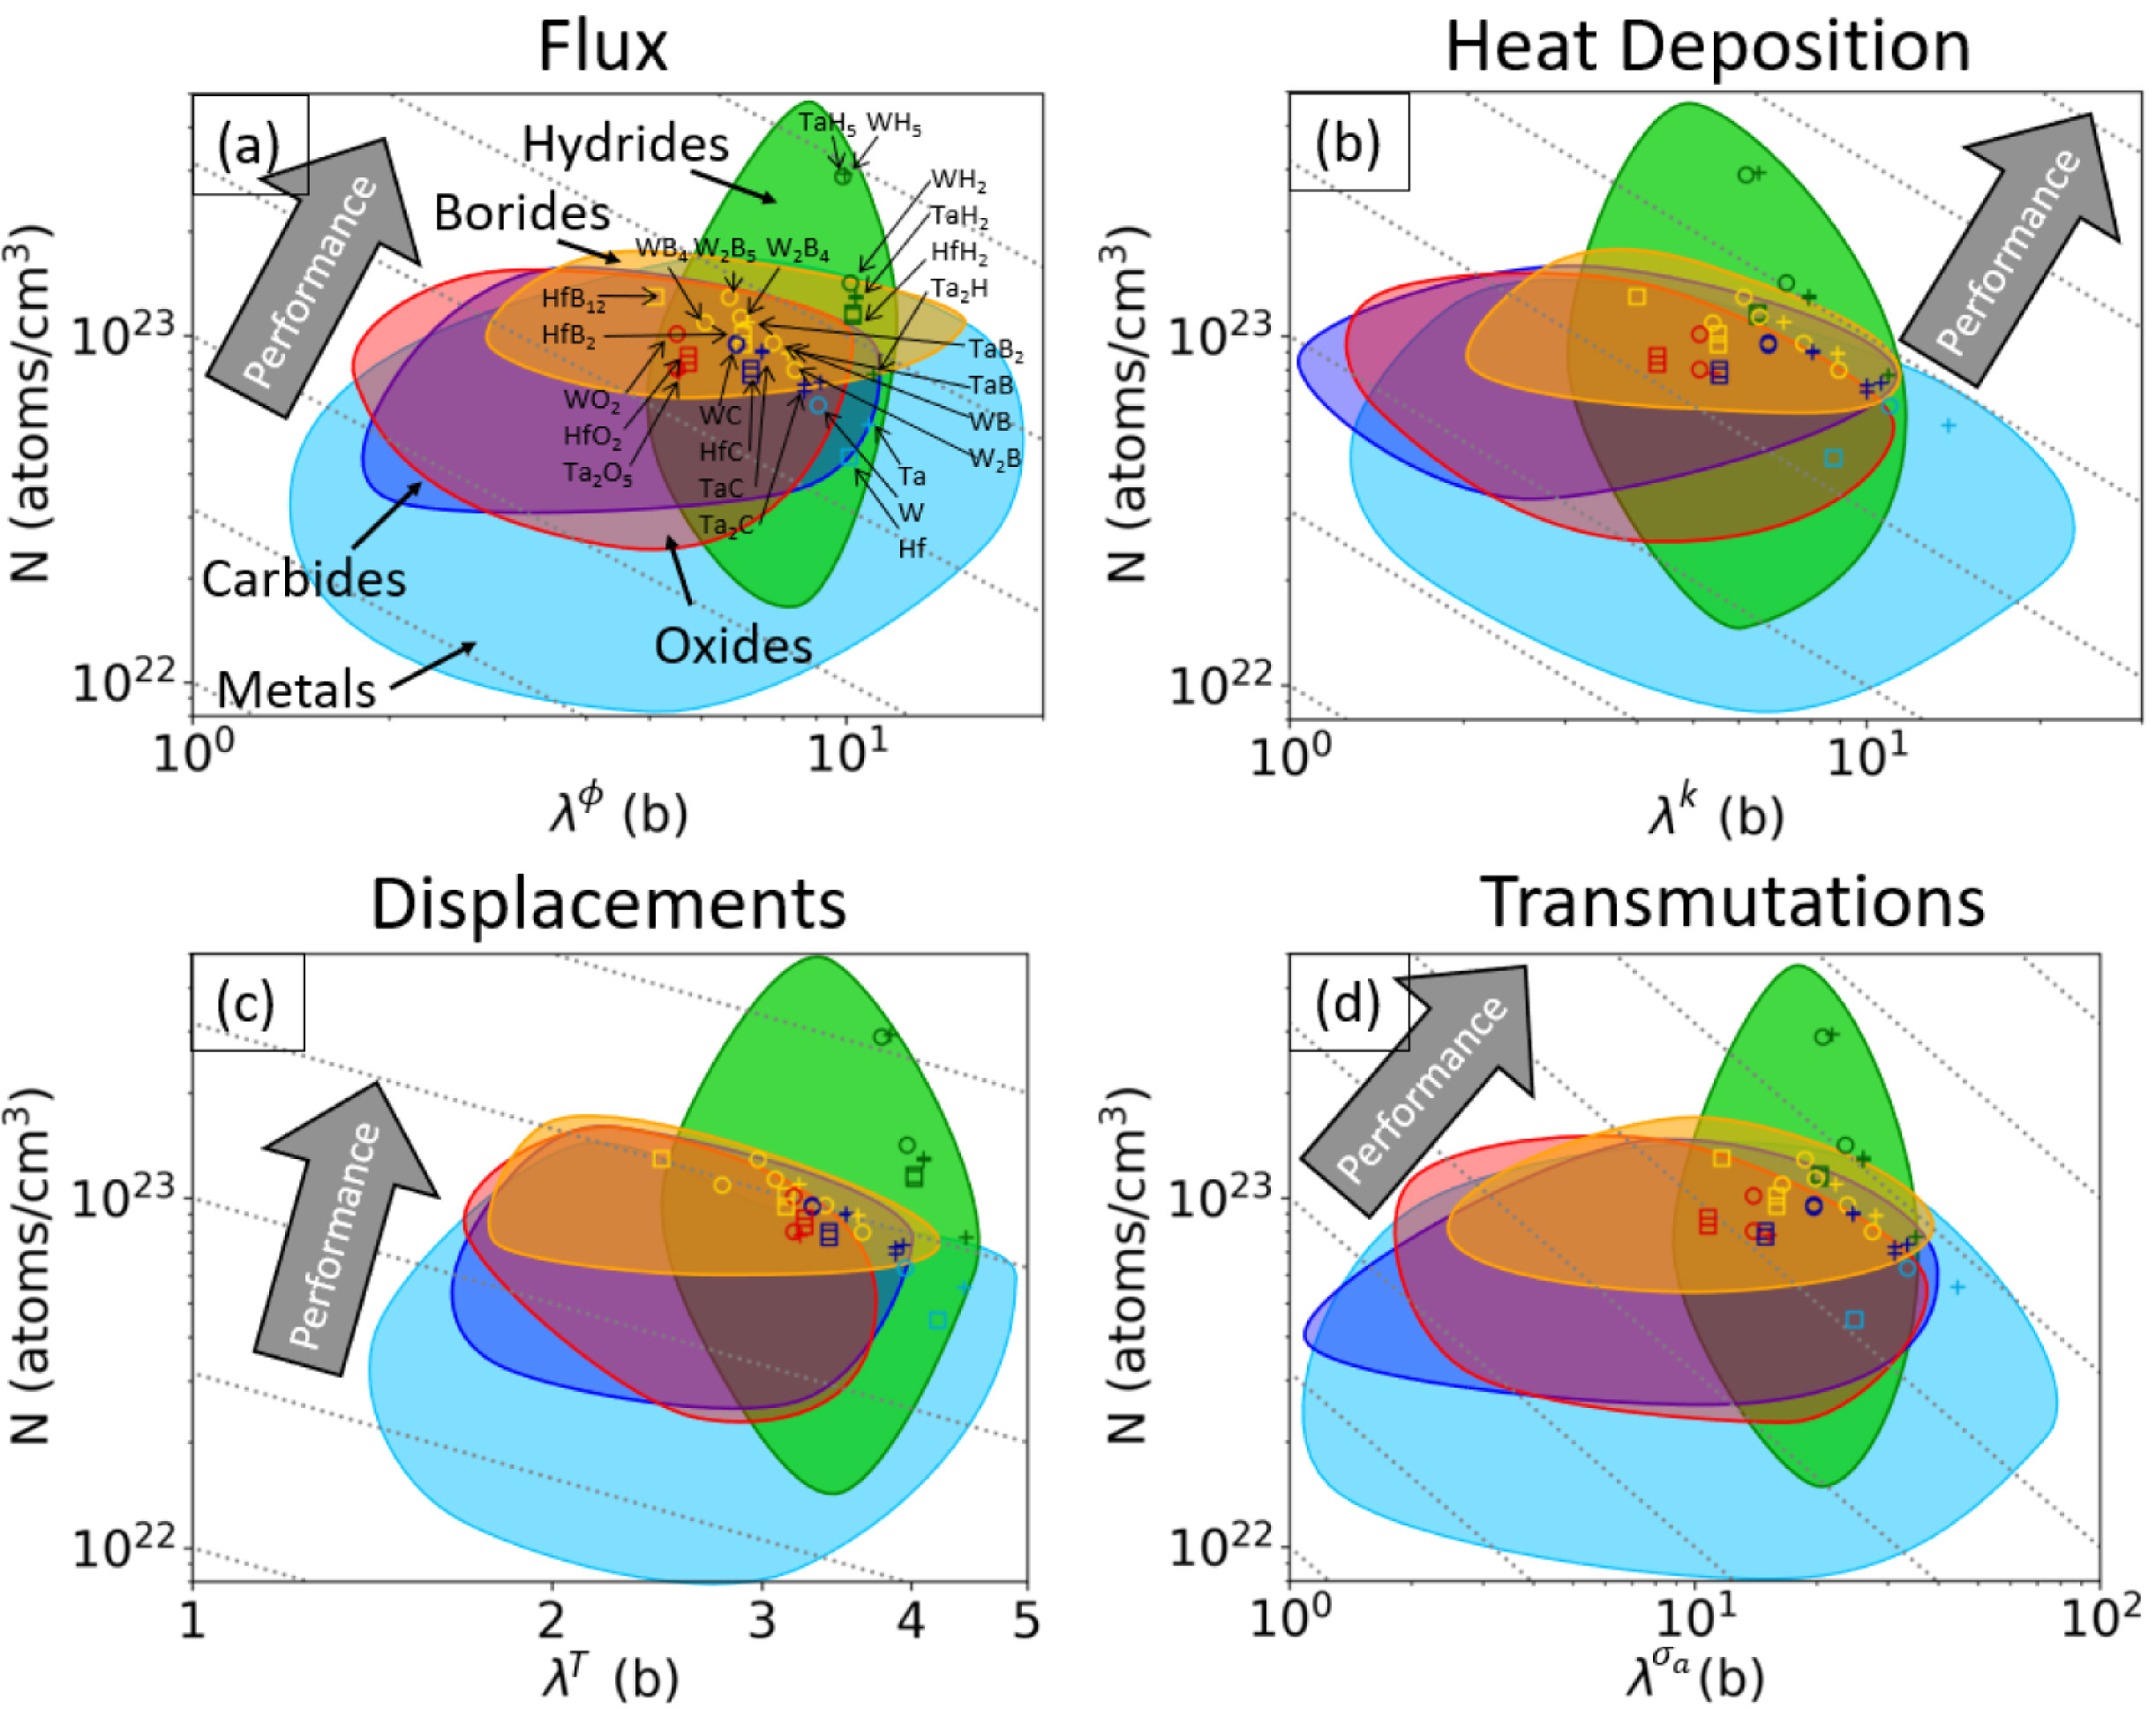
\includegraphics[width=0.7\linewidth]{../images/graph-3.jpg}
    \caption{Selección de materiales para blindaje de espesor mínimo. \cite{Brand2025Material}}
  \end{figure}
\end{frame}

\begin{frame}
  \frametitle{El Material Óptimo para el Reactor de Fusión}
  \begin{block}{Recordando el Objetivo}
    Buscamos el material con el mayor \textbf{Índice de Material} para minimizar el espesor:
    $$ \mathcal{M}_{1} = N \cdot \lambda_{eff} $$
  \end{block}

  \begin{alertblock}{Los Candidatos Ganadores}
    Los \textbf{Hidruros Metálicos} y los \textbf{Boruros} (como el Boruro de Tungsteno) son los mejores materiales.
  \end{alertblock}
  \begin{block}{¿Por Qué Son los Mejores? La Razón detrás de $\mathcal{M}_{1}$}
    \begin{itemize}
      \item \textbf{Hidruros Metálicos}: Su ventaja es una \textbf{densidad atómica ($N$) extremadamente alta}. Dominan el componente '$N$' del índice.
      \item \textbf{Boruros}: Ofrecen un \textbf{excelente balance}. Tienen buena densidad atómica ($N$) y un \textbf{coeficiente de atenuación ($\lambda_{eff}$) muy efectivo}.
    \end{itemize}
  \end{block}
\end{frame}
